\subsection{Implementation}
When divided into two main packages the runtime process simplifies to following steps:
\begin{itemize}
    \item Kinematics: Scans the target provides requested image and pose pairs to the vision package
    \item Vision: Processes aforementioned inputs to provide 3-float vector corresponding the position of the target point, accompanied by information on the possible approach orientation for insertion.
    \item Kinematics: Inserts the needle in to the target point, while keeping the needle on a straight line when inside the phantom.
\end{itemize}

The interaction between these two packages can be illustrated with the Figure \ref{overview}.

\begin{figure}
    \label{overview}
    \caption{Overview of the package interaction}
    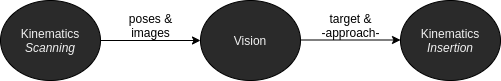
\includegraphics[width=0.5\textwidth]{images/overview}
\end{figure}


To utilize ROS and already existing Franka ROS Library the kinematics package is formed by the following nodes:
\begin{itemize}
    \item simple\_scanner: Employs the scanning routine around the target point to generate image and pose pairs necessary for vision. Holds SphericalScanner class.
    \item simple\_capture: Communicates with scanner node to save necessary information at every stop. Holds ImageCapture class.
    \item simple\_inserter: Manages the insertion procedure given a target point and a peak point. Holds Inserter class.
    \item simple\_planner: Trajectory planner node, plans and publishes the plans on desired control frequency given the goal pose in homogenous transformation. Holds TrajectoryPlanner class.
    \item simple\_goal: A goal definer for debugging purposes. It is created to test the kinematics application not depending on the state of the vision package. Holds GoalSetter class.
\end{itemize}
These active nodes are utilizing the following modules
\begin{itemize}
    \item simple\_node: Holds the Communicative\_Node parent class which is inherited by most of the classes in this package. It maps all the necessary topics while keeping track of whether the process is on simulation. It also has some commonly used methods by most of the other modules such as waiting for execution or getting joint states.
    \item simple\_robot: Holds Robot class that is imported whenever forward kinematics is needed to be employed. It uses the inherent links that are provided by manufacturer and also necessary end effectors which all are broadcasted via tf package from ROS.
    \item simple\_ik: Holds Inverse\_Kinematics class which is executed whenever there is need of inverse kinematics calculation.
    \item simple\_quintics: Includes mostly static mathematical methods that are necessary to plan a trajectory with quintic polynomials.
    \item simple\_cartographer: Helps the trajectory planner when it needs to make end effector point at some point during scanning or insertion processes.
\end{itemize}

A diagram to help visualize the kinematics package can be found in Appendix, Figure \ref{app_overview}.

The entire process can be summarized as
\begin{itemize}
    \item Scanner node starts a spherical scan pattern around the approximate target point whilst directing the camera towards it with the help of Cartographer. During which there is a checkerboard for calibration purposes.
    \item Capture node captures images and poses to pass on Vision package.
    \item Receiving the target point and approach direction Inserter class first peaks at the target point where it can insert the needle on a straight line, then inserts it to the target.
\end{itemize}
During this process Cartographer helps directing the end effector to the desired orientation, Robot class tracks the provided and developped coordinate frames and joint limits, inverse kinematics  calculates the joint states that are needed to be reached for the target point at each step. All of which are passed to the planner which outputs a plan quantized with the control frequency, or in case of insertion fed directly to the command topic of robot.


The entire implementation of this package is done on most recent versions of both Python and ROS, which during the time of the study were 3.9 and Noetic respectively.
Indeed the provided robot framework runs on the Python 2.7 and ROS Kinetic, which has potential to pose a problem via incompatibility.
Although at the end flexible ROS architecture allowed us to run the package on another computer on the same network and communicate controller via topics.
One more implementation note is the use of a modified fork of franka\_ros package.
To be able to communicate the current execution state, franka\_ros package is modified accordingly and stored in a separate fork from the original clone that was provided.